\subsection{Hybrid STM/HTM}\label{sec:hybrid}
\begin{figure}[t]\begin{center}%
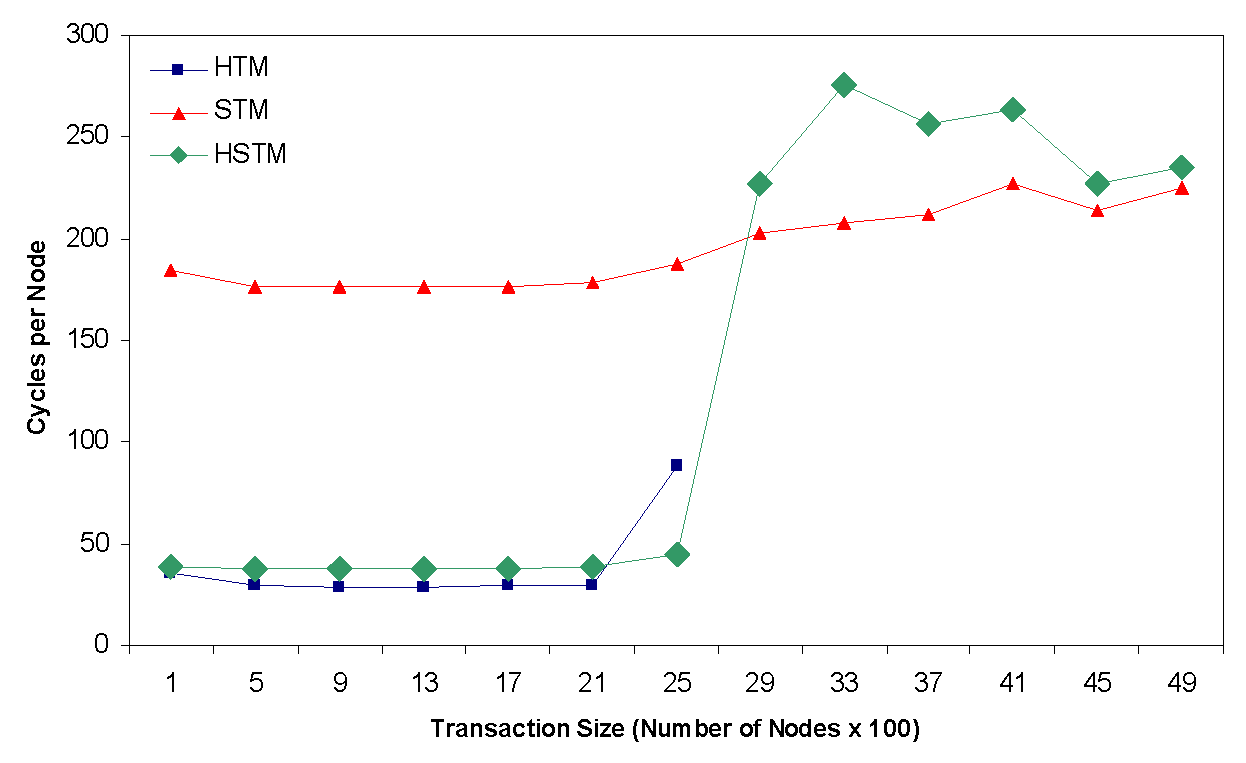
\includegraphics[width=3.25in,clip=true]{Figures/sean_lie_6b.eps}%
\end{center}%
\caption{Performance (in cycles per node push on a simple queue
  benchmark) of LTM~\cite{AnanianAsKuLeLi04} (HTM), the
  object-based system presented in this paper (STM) and a hybrid
  scheme (HSTM).}%
\label{fig:hybrid}%
\end{figure}
It is worth considering if a low-level HTM can yield benefits other
than efficient implementations of large-object operations.  In fact,
\figref{hybrid} presents research showing that we can combine the
strengths of our object-based software transaction system with a
fast bounded-size HTM.  In the figure, combining the systems is done
in the most simple-minded way: all transactions are begun in
LTM~\cite{AnanianAsKuLeLi04},
and after any abort the transaction is restarted in the
object-based software system.  The field flag mechanism described in
\secref{flagfield} ensures that software transactions properly abort
conflicting hardware transactions; hardware transactions must perform
the \texttt{ReadNT} and \texttt{WriteNT} algorithms for a slight
overhead (as shown in the figure).
